% Options for packages loaded elsewhere
\PassOptionsToPackage{unicode}{hyperref}
\PassOptionsToPackage{hyphens}{url}
\PassOptionsToPackage{dvipsnames,svgnames,x11names}{xcolor}
%
\documentclass[
  10pt,
  twocolumn]{article}
\usepackage{amsmath,amssymb}
\usepackage{iftex}
\ifPDFTeX
  \usepackage[T1]{fontenc}
  \usepackage[utf8]{inputenc}
  \usepackage{textcomp} % provide euro and other symbols
\else % if luatex or xetex
  \usepackage{unicode-math} % this also loads fontspec
  \defaultfontfeatures{Scale=MatchLowercase}
  \defaultfontfeatures[\rmfamily]{Ligatures=TeX,Scale=1}
\fi
\usepackage{lmodern}
\ifPDFTeX\else
  % xetex/luatex font selection
\fi
% Use upquote if available, for straight quotes in verbatim environments
\IfFileExists{upquote.sty}{\usepackage{upquote}}{}
\IfFileExists{microtype.sty}{% use microtype if available
  \usepackage[]{microtype}
  \UseMicrotypeSet[protrusion]{basicmath} % disable protrusion for tt fonts
}{}
\makeatletter
\@ifundefined{KOMAClassName}{% if non-KOMA class
  \IfFileExists{parskip.sty}{%
    \usepackage{parskip}
  }{% else
    \setlength{\parindent}{0pt}
    \setlength{\parskip}{6pt plus 2pt minus 1pt}}
}{% if KOMA class
  \KOMAoptions{parskip=half}}
\makeatother
\usepackage{xcolor}
\usepackage[margin=0.7in]{geometry}
\usepackage{longtable,booktabs,array}
\usepackage{calc} % for calculating minipage widths
% Correct order of tables after \paragraph or \subparagraph
\usepackage{etoolbox}
\makeatletter
\patchcmd\longtable{\par}{\if@noskipsec\mbox{}\fi\par}{}{}
\makeatother
% Allow footnotes in longtable head/foot
\IfFileExists{footnotehyper.sty}{\usepackage{footnotehyper}}{\usepackage{footnote}}
\makesavenoteenv{longtable}
\usepackage{graphicx}
\makeatletter
\def\maxwidth{\ifdim\Gin@nat@width>\linewidth\linewidth\else\Gin@nat@width\fi}
\def\maxheight{\ifdim\Gin@nat@height>\textheight\textheight\else\Gin@nat@height\fi}
\makeatother
% Scale images if necessary, so that they will not overflow the page
% margins by default, and it is still possible to overwrite the defaults
% using explicit options in \includegraphics[width, height, ...]{}
\setkeys{Gin}{width=\maxwidth,height=\maxheight,keepaspectratio}
% Set default figure placement to htbp
\makeatletter
\def\fps@figure{htbp}
\makeatother
\setlength{\emergencystretch}{3em} % prevent overfull lines
\providecommand{\tightlist}{%
  \setlength{\itemsep}{0pt}\setlength{\parskip}{0pt}}
\setcounter{secnumdepth}{-\maxdimen} % remove section numbering
\newlength{\cslhangindent}
\setlength{\cslhangindent}{1.5em}
\newlength{\csllabelwidth}
\setlength{\csllabelwidth}{3em}
\newlength{\cslentryspacingunit} % times entry-spacing
\setlength{\cslentryspacingunit}{\parskip}
\newenvironment{CSLReferences}[2] % #1 hanging-ident, #2 entry spacing
 {% don't indent paragraphs
  \setlength{\parindent}{0pt}
  % turn on hanging indent if param 1 is 1
  \ifodd #1
  \let\oldpar\par
  \def\par{\hangindent=\cslhangindent\oldpar}
  \fi
  % set entry spacing
  \setlength{\parskip}{#2\cslentryspacingunit}
 }%
 {}
\usepackage{calc}
\newcommand{\CSLBlock}[1]{#1\hfill\break}
\newcommand{\CSLLeftMargin}[1]{\parbox[t]{\csllabelwidth}{#1}}
\newcommand{\CSLRightInline}[1]{\parbox[t]{\linewidth - \csllabelwidth}{#1}\break}
\newcommand{\CSLIndent}[1]{\hspace{\cslhangindent}#1}
\ifLuaTeX
  \usepackage{selnolig}  % disable illegal ligatures
\fi
\IfFileExists{bookmark.sty}{\usepackage{bookmark}}{\usepackage{hyperref}}
\IfFileExists{xurl.sty}{\usepackage{xurl}}{} % add URL line breaks if available
\urlstyle{same}
\hypersetup{
  pdftitle={Ochrell: Continuous Spectral Reconstruction and Optical-Strength Priors for RGB Pigment Mixing},
  pdfauthor={Ochrell project --- independent implementation study},
  colorlinks=true,
  linkcolor={Maroon},
  filecolor={Maroon},
  citecolor={Blue},
  urlcolor={Blue},
  pdfcreator={LaTeX via pandoc}}

\title{Ochrell: Continuous Spectral Reconstruction and Optical-Strength
Priors for RGB Pigment Mixing}
\author{Ochrell project --- independent implementation study}
\date{29 September 2026 · research release 0.2}

\setlength{\emergencystretch}{2em}
\sloppy
\begin{document}
\maketitle

\hypertarget{abstract}{%
\section{Abstract}\label{abstract}}

RGB colors do not uniquely identify reflectance spectra or the
absorption and scattering coefficients of paint. A useful digital
pigment mixer must therefore choose explicit priors as well as reproduce
its inputs. We investigate a mathematical revision of an independently
implemented Rust Kubelka--Munk mixer, without acquiring pigment
measurements or fitting to another engine's outputs. Three bounded,
smooth reflectance anchors and their complements support a continuous
linear-RGB reconstruction. A geometric-mean optical normalization
assigns separate absorption and scattering strengths; a small
linear-light residual restores the source color. The resulting encoder
has no nonlinear optimization or lookup table at runtime. On 10000
seeded colors, mean uncorrected reconstruction error falls from 11.5 to
0.072 CIEDE2000. In an independent blue/yellow color-family diagnostic,
green-dominant midpoint frequency increases from 38.4\% to 80.8\%. The
fast 41-band model differs from the 81-band double-precision reference
by mean 0.00352 and maximum 0.0999 CIEDE2000 over 10000 random mixtures.
Median throughput on the recorded host is 1.39 million complete RGB
mixtures per second, or 4.37 million with cached optical states.
White-tint hue shifts decrease, but latent storage grows and uncached
mixing is slower than the preceding LUT implementation. These results
establish numerical and design improvements within a synthetic model,
not physical accuracy for a particular paint formulation.

\hypertarget{introduction}{%
\section{1. Introduction}\label{introduction}}

A digital painter expects color mixing to resemble material interaction:
yellow and blue should often produce green; adding white should lighten
a color with characteristic changes in chroma; complementary colors
should lose saturation. Neither encoded RGB averaging nor additive
linear-light interpolation models absorption and scattering within
paint. A perceptual color space regularizes perceived transitions, but
also does not establish a material interpretation.

The main ambiguity arises before mixing. Three RGB components constrain
only three integrals of a reflectance spectrum. A spectrum can be
selected by regularization, yet opaque reflectance still supplies only
the ratio of absorption to scattering. Different absolute optical
strengths can preserve the isolated color and produce different
mixtures. Mathematical design can improve a general RGB painting model
without new measurements, but cannot identify the actual paint that
generated an arbitrary RGB color.

Our preceding implementation used an eight-component synthetic pigment
palette, constrained nonlinear inversion, a reconstruction residual and
a tetrahedral encoder LUT. Its default yellow/blue example produced
green, but additional tests revealed a dark blue/yellow pair that mixed
to blue-gray, a muted cyan/magenta mixture and peach-shifting red/white
tints. Large residuals and disagreement between interpolated and
directly optimized recipes exposed a deeper issue: endpoint accuracy
concealed a weak and sometimes unstable material representation.

We compare three responses: refitting the finite pigment palette,
directly reconstructing reflectance with conventional scattering
assumptions, and reconstructing reflectance with a declared
optical-strength prior. The last is selected on recorded diagnostic
evidence. This changes the meaning of the basis: it becomes a
colorimetric reconstruction basis rather than a palette of identifiable
physical ingredients. We retain the old implementation and unsuccessful
alternatives so that the change can be examined rather than inferred
from favorable images alone.

Our contributions are an independently generated continuous
reconstruction and optical-state representation; a dependency-free Rust
implementation with separate precision/sampling paths; and a
reproducible evaluation of reconstruction, trajectories, tints,
sampling, parameter choices and performance. We do not claim invention
of spectral upsampling, Kubelka--Munk mixing or residual correction. We
do not claim measured paint fidelity, numerical compatibility with
Mixbox, or a statistically established preference among artists.

\begin{figure*}[t]
\centering
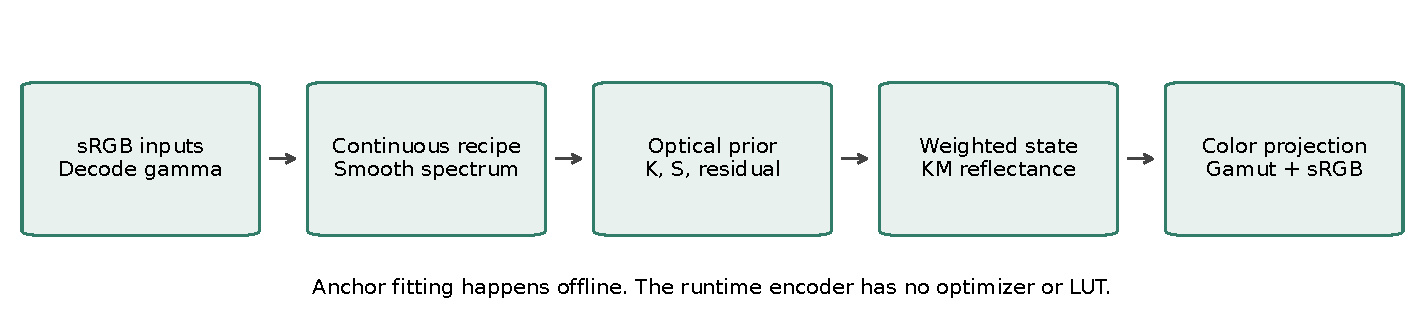
\includegraphics[width=0.94\textwidth,height=0.72\textheight,keepaspectratio]{figures/pipeline.pdf}
\caption{The default pipeline. Anchor fitting is offline;
input-dependent inversion is explicit and continuous.}
\end{figure*}

\hypertarget{related-work}{%
\section{2. Related work}\label{related-work}}

Kubelka and Munk's two-flux theory and Kubelka's later development
provide approximate relationships between diffuse reflectance,
absorption and scattering (Kubelka and Munk 1931; Kubelka 1948). Haase
and Meyer apply pigment optics to graphics and paint-oriented color
selection (Haase and Meyer 1992). Curtis et al.~combine optical layers
with separate watercolor transport (Curtis et al. 1997). These
precedents distinguish homogeneous color mixing from the larger
simulation of thickness, substrate and fluid motion.

Spectral reconstruction from RGB is underdetermined. Smits demonstrates
compact reflectance bases (Smits 1999); Burns examines smoothness-based
reconstruction (Burns 2020); Jakob and Hanika construct an efficient
low-dimensional space of bounded spectra (Jakob and Hanika 2019). Our
construction follows the broad basis and smoothness motivations, but
fits its own spectra using the objective stated below. None of these
colorimetric methods, by itself, establishes the independent scattering
strength needed for pigment mixing.

Sochorová and Jamriška's contribution goes beyond applying classical
K--M equations: their practical RGB interface uses a latent pigment
representation, additive color residuals, surrogate-pigment treatment of
gamut limitations and acceleration (Sochorová and Jamriška 2021). Their
published representation motivates the compatibility residual used in
both of our versions. We do not use their proprietary coefficients,
implementation artifacts or lookup tables. The present revision stores
wavelength-wise K and S rather than concentrations over our previous
finite palette. This avoids that palette's nonlinear inverse, while
increasing state size and giving up ingredient identification.

Pigmento studies pigment-oriented image decomposition and editing, a
different problem from a stateless per-color encoder (Tan et al. 2017).
RYB-inspired interpolation provides an intuitive color-control
alternative without identifying spectra (Gossett and Chen 2004).
Neugebauer-type models are appropriate to area coverages and overprinted
layers rather than a direct replacement for homogeneous pigment-volume
mixing (Hébert and Hersch 2015). We retain sRGB, linear RGB and OKLab
(Ottosson 2020) as inexpensive baselines.

Spectral.js is an open-source RGB pigment-like mixer with a spectral
reconstruction and K--M formulation (Spectral.js contributors, n.d.). We
compare its public version 3.0.0 API outputs and previously captured
Mixbox demonstration outputs after selecting our model. Similarity to
these engines is a descriptive comparison, not a measurement of physical
truth. No external mixing implementation, spectra or output samples
enter our fitting objective.

\hypertarget{color-and-optical-background}{%
\section{3. Color and optical
background}\label{color-and-optical-background}}

\hypertarget{colorimetric-projection}{%
\subsection{3.1 Colorimetric projection}\label{colorimetric-projection}}

Let \(r_j\) denote reflectance at wavelength \(\lambda_j\), \(E_j\) the
D65 illuminant and \(\bar{x}_j,\bar{y}_j,\bar{z}_j\) the CIE 1931
two-degree color-matching functions. Trapezoidal quadrature gives

\[[X,Y,Z]^T = k\sum_j h_j E_j r_j[\bar{x}_j,\bar{y}_j,\bar{z}_j]^T,\]

where \(h_j\) includes interval and endpoint weights and
\(k^{-1}=\sum_jh_jE_j\bar{y}_j\). The reference uses 380--780 nm at 5 nm
intervals. The input tables are the attributed, modified Colour-package
subset documented in the repository, rather than an unmodified copy of
current official CIE files (Colour Developers, n.d.; International
Commission on Illumination 2019b, 2019a).

A fixed XYZ-to-linear-sRGB matrix gives a projection
\(A\in\mathbb{R}^{3\times N}\). Each RGB quadrature column is
additionally normalized to make a unit reflector project exactly to
\([1,1,1]\). This numerical white correction is part of our model. It
should not be confused with exact unmodified standard colorimetry. The
normalized Y quadrature is denoted \(y_j\).

For encoded sRGB channel \(u\), linear intensity is \(x=u/12.92\) below
or at 0.04045, and \(x=((u+0.055)/1.055)^{2.4}\) otherwise (World Wide
Web Consortium, n.d.). Reflectance, optical mixing and residual addition
occur before display encoding. Inputs are finite bounded sRGB, not HDR
emission or premultiplied colors.

\hypertarget{infinite-thickness-km}{%
\subsection{3.2 Infinite-thickness K--M}\label{infinite-thickness-km}}

With absorption \(K_j\geq0\) and scattering \(S_j>0\), define
\(q_j=K_j/S_j\). The opaque reflectance and its inverse are

\[r_j=\frac{1}{1+q_j+\sqrt{q_j(q_j+2)}},\qquad q_j=\frac{(1-r_j)^2}{2r_j}.\]

The reciprocal form avoids subtractive cancellation in the usual
expression \(1+q-\sqrt{q^2+2q}\). We assume linear mixing of K and S
with normalized material amounts. This is a selected homogeneous diffuse
model; interactions between particles, binder changes and surface
reflections are outside it.

Multiplying both K and S of one component by a positive scalar preserves
its isolated reflectance but changes its influence in mixtures.
Therefore an RGB-only mixer must select both a spectral metamer and an
optical-strength convention. Exact endpoint reconstruction cannot
resolve this ambiguity.

\hypertarget{method}{%
\section{4. Method}\label{method}}

\hypertarget{offline-spectral-basis}{%
\subsection{4.1 Offline spectral basis}\label{offline-spectral-basis}}

We fit only the three linear-sRGB primary anchors
\(p\in\{(1,0,0),(0,1,0),(0,0,1)\}\). Let \(\epsilon=0.001\),
\(\sigma(z)=1/(1+\exp(-z))\) and \(D\) be the unscaled first-difference
operator on the reference grid. Solve

\[\min_z \left\|A[\epsilon+(1-2\epsilon)\sigma(z)]-p\right\|_2^2+\lambda^2\|Dz\|_2^2,\]

with \(\lambda=0.001\). The logistic parameterization bounds reflectance
strictly away from singular black and white. Logit smoothing encourages
transitions across wavelength without prescribing measured pigment
absorption bands. The reflectance floor limits achievable anchor
accuracy; the residual addresses the remaining error.

Initialization is a bounded linear least-squares reflectance fit with a
0.01 first-difference penalty. Its normalized reflectance is clipped to
\([10^{-4},1-10^{-4}]\) before conversion to logit coordinates. SciPy
least squares uses an analytic Jacobian, termination tolerances
\(10^{-12}\) and at most 2,000 evaluations. Convergence records and a
generated-basis checksum are saved. We make no claim of a unique
spectrum or globally optimal nonlinear solution.

Given fitted primary spectra \(B_R,B_G,B_B\), define complements
\(B_C=1-B_R\), \(B_M=1-B_G\), \(B_Y=1-B_B\), plus constant
\(B_W=1-\epsilon\) and \(B_K=\epsilon\). These are eight reconstruction
functions generated from three solves. Their coefficients are
independent of other mixing libraries. Figure 2 shows their shapes and
one inferred optical state.

\begin{figure*}[t]
\centering
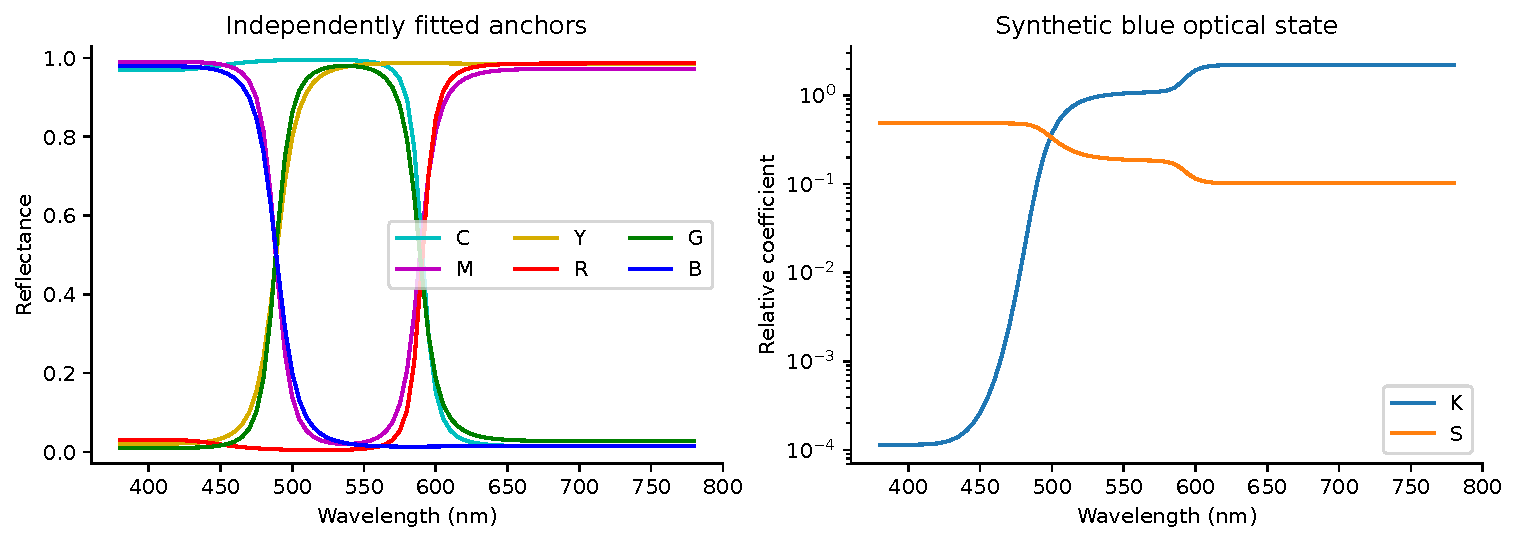
\includegraphics[width=0.94\textwidth,height=0.72\textheight,keepaspectratio]{figures/spectra.pdf}
\caption{Fitted reflectance anchors and the inferred K/S state for sRGB
(20,70,255). The spectra are mathematical priors, not pigment
measurements.}
\end{figure*}

\hypertarget{explicit-continuous-reconstruction}{%
\subsection{4.2 Explicit continuous
reconstruction}\label{explicit-continuous-reconstruction}}

For linear RGB \(x\), let \(l\leq m\leq h\) be its sorted channel
values. Place weight \(l\) on white, \(1-h\) on black, \(m-l\) on the
secondary complementary to the minimum channel, and \(h-m\) on the
maximum-channel primary. The four weights are nonnegative and sum to
one. Reconstruct \(r=\sum_i w_iB_i\).

This is a piecewise-affine cube decomposition. At a channel-order
boundary, the switching term has zero weight or agrees with the limiting
recipe, so the spectrum is continuous. The first derivative need not be
continuous. Since all anchors lie in \([\epsilon,1-\epsilon]\), every
reconstructed spectrum satisfies the same bounds. There is no
input-dependent iterative optimization and no encoder LUT. The
quantities \(w_i\) are reconstruction weights, not asserted physical
pigment concentrations.

\hypertarget{optical-strength-prior-and-white-behavior}{%
\subsection{4.3 Optical-strength prior and white
behavior}\label{optical-strength-prior-and-white-behavior}}

After reconstructing \(r\), calculate \(q\) using K--M inversion and
\(Y=\sum_jy_jr_j\). Define neutral scattering normalization
\(s_n=2Y/(1+Y^2)\). For a neutral spectrum, this equals \(1/(1+q)\). Our
explored family is

\[S_j=\eta(1+q_j)^{-\beta}s_n^{1-\beta},\quad K_j=q_jS_j,\]

\[\eta=1+(w_{\mathrm{white}}-1)\min(x).\]

At \(\beta=0\), S is wavelength-independent and adjusted to the
spectrum's luminance. At \(\beta=1\), \(K_j+S_j=\eta\) independently at
every wavelength. We choose \(\beta=1/2\), the geometric mean of these
normalizations, and \(w_{\mathrm{white}}=2\). The implementation needs a
square root rather than a general fractional power.

The scalar \(\eta\) increases optical strength with the color's
neutral-white component without changing its isolated K/S ratio. This is
a declared tinting prior. It is not a measured titanium-white scattering
coefficient, and the same RGB color from two different real paints need
not follow it. Parameter experiments below show why neither constant S
nor a pure per-band budget was adequate for our diagnostics.

\hypertarget{persistent-optical-states-and-residuals}{%
\subsection{4.4 Persistent optical states and
residuals}\label{persistent-optical-states-and-residuals}}

Encode the state \(z=(K,S,e)\), where \(e=x-Ar\) is a linear-RGB
residual. For normalized nonnegative amounts \(\alpha_i\), blend all
components:

\[K'=\sum_i\alpha_iK_i,\quad S'=\sum_i\alpha_iS_i,\quad e'=\sum_i\alpha_i e_i.\]

Apply K--M reflectance to \(K'/S'\) and return \(Ar'+e'\) before gamut
mapping. At a source endpoint, this reproduces x algebraically. Public
pair mixing additionally returns the exact supplied endpoint objects.
Finite-precision encode/decode reconstruction remains a separate test.
The small residual does not certify that the inferred spectrum is
physically correct.

Weighted optical-state mixtures are associative up to rounding when
aggregate weights carry the total amount of each group. Decoding a
mixture to RGB and re-encoding it loses spectral information and is not
associative. This distinction matters for brush engines: repeatedly
mixing only display colors does not retain the previous material state.

\hypertarget{gamut-mapping-and-continuity}{%
\subsection{4.5 Gamut mapping and
continuity}\label{gamut-mapping-and-continuity}}

We retain the earlier neutral-axis gamut compression. Compute
\(L=\mathrm{clamp}(0.2126x_r+0.7152x_g+0.0722x_b,0,1)\) and select the
largest \(a\in[0,1]\) placing \(L+a(x-L)\) inside the RGB cube. The map
is identity in gamut and preserves this luminance when it is in range;
it does not preserve perceptual hue exactly.

All ideal-arithmetic stages are continuous on the bounded input domain.
Strictly positive scattering prevents division singularities. This
establishes continuity, not constant perceptual speed, monotone hue or
monotone chroma. In particular, OKLab's cube root is highly sensitive
near black. Numerical trajectories and endpoint refinement are reported
separately from the structural argument.

\hypertarget{reference-and-fast-implementation}{%
\section{5. Reference and fast
implementation}\label{reference-and-fast-implementation}}

The reference uses 81 wavelength samples at 5 nm and f64 optical
arithmetic. The fast path uses 41 samples at 10 nm and f32 arrays, with
f64 transfer functions, residual addition and final gamut mapping. A
shared Rust kernel keeps their equations aligned; an independent NumPy
implementation provides an additional check. We report both
spectral-discretization error and same-grid arithmetic error.

The default mixer is stateless and zero-sized. Encoding, pair mixing and
weighted accumulation require no heap allocation or platform-specific
calls. Weighted accumulation uses f64 before storing the result at the
selected precision. The crate forbids unsafe code and has no Cargo
dependencies. Python, SciPy, Colour and Matplotlib are offline
fitting/evaluation tools. The core design is compatible with a WASM
integration path; browser performance is not measured here.

A fast optical state occupies 340 bytes, versus 44 for the legacy
concentration-plus-residual state. The new basis and fast quadrature
occupy approximately 1968 bytes as numeric arrays; the default no longer
parses the legacy 1149992-byte LUT. Legacy assets remain in the research
repository. Storing a state per canvas pixel is consequently more
expensive even though startup and encoder-table memory are reduced.
Brush-color caching or sparse material storage may be preferable.

The final encoder integrates its reconstructed reflectance directly when
computing the residual. In exact arithmetic, subsequent K--M inversion
recovers that reflectance. This removes redundant square roots at the
cost of small measured f32 roundoff. The optimized implementation
retains exact public pair endpoints and validates the encode/decode
round trip. Explicit SIMD, GPU execution and compression are future
work.

\hypertarget{experimental-methodology}{%
\section{6. Experimental methodology}\label{experimental-methodology}}

We use 10000 uniformly sampled encoded-sRGB colors and 10000 random
pairs with uniformly sampled t, generated by the recorded xorshift64
sequence with seed 20260930. Uniform encoded RGB is not uniform
perceptual color or a model of artists' usage. The same samples compare
the old default with the new default. Reconstruction is evaluated both
with and without residual correction using CIEDE2000 (Sharma, Wu, and
Dalal 2005). OKLab distance multiplied by 100 is used for local
trajectory diagnostics; it is not interchangeable with CIEDE2000.

Thirteen canonical pairs include ordinary and saturated primaries,
complements, white and black, and the dark-blue/yellow failure case from
the earlier comparison. Each has 1001 samples. We also evaluate 200
random trajectories, 5,000 input perturbations of \(10^{-5}\) in one
encoded channel, and 1,024 white tints at the same dense spacing. Tint
hue shifts are compared only where source chroma exceeds 0.04 and both
models' midpoint chroma exceeds 0.02, giving 957 common eligible cases.
Hue retention is a design diagnostic, not a general physical law.

Parameter selection used 512 blue/yellow pairs and 1,024 white-tint
colors generated independently in NumPy with seed 20260930. Yellow hues
span 45--75 degrees, blue hues 220--255 degrees; saturation spans
0.6--0.95, yellow value 0.5--1 and blue value 0.2--1. A held-out
2,048-pair family uses seed 20261001. We call a midpoint green-dominant
when its green channel exceeds red and blue and its OKLab chroma is at
least 0.03. This is a deliberately simple algebraic criterion. Not every
real pigment pair in these RGB ranges would necessarily satisfy it.

Timings use 7 repetitions of 100000 operations, varying among 256 seeded
colors and 997 interpolation values. Rust \texttt{black\_box} prevents
constant folding. Runs are single-threaded, release mode, LTO disabled
and one codegen unit, without target-cpu=native. The host reports AMD
EPYC 9V74 80-Core Processor; compiler is rustc 1.75.0 (82e1608df
2023-12-21) (built from a source tarball). Raw repetitions and full
environment are stored. Cached timings include interpolation and display
decoding but exclude the two input encodes. CPU frequency, cache
conditions and shared-host load limit transferability.

\hypertarget{external-comparison-protocol}{%
\subsection{6.1 External comparison
protocol}\label{external-comparison-protocol}}

The external comparison is deliberately frozen. Mixbox observations are
median pixels from the official gradient demo's JPEG captures at t=0.25,
0.5 and 0.75 for the same thirteen pairs. The 39-point sRGB control has
mean approximately 0.286 and maximum 0.804 CIEDE2000 capture
discrepancy. Mixbox comparisons are therefore approximate observations,
not SDK equality tests.

Spectral.js 3.0.0 supplies 401 public-API samples per pair, using
default tinting strength 1 and gamut method \texttt{map}; outputs are
its native 8-bit sRGB values. Its version, package checksum, invocation
and endpoint checks are frozen with the data. We use no external
spectra, coefficients or implementation internals, and neither
comparator enters candidate fitting or selection. The bundled baseline
comparison archive supports reanalysis of the observations; reacquiring
a future live demo would be a new experiment.

\hypertarget{results}{%
\section{7. Results}\label{results}}

\hypertarget{reconstruction-and-approximation}{%
\subsection{7.1 Reconstruction and
approximation}\label{reconstruction-and-approximation}}

\begin{table*}[t]
\caption{Source reconstruction (CIEDE2000), identical sample set.}
\centering\small
\begin{tabular}{@{}
  >{\raggedright\arraybackslash}p{(\textwidth - 10\tabcolsep) * \real{0.1667}}
  >{\raggedright\arraybackslash}p{(\textwidth - 10\tabcolsep) * \real{0.1667}}
  >{\raggedright\arraybackslash}p{(\textwidth - 10\tabcolsep) * \real{0.1667}}
  >{\raggedright\arraybackslash}p{(\textwidth - 10\tabcolsep) * \real{0.1667}}
  >{\raggedright\arraybackslash}p{(\textwidth - 10\tabcolsep) * \real{0.1667}}
  >{\raggedright\arraybackslash}p{(\textwidth - 10\tabcolsep) * \real{0.1667}}@{}}
\toprule\noalign{}
\begin{minipage}[b]{\linewidth}\raggedright
Reconstruction
\end{minipage} & \begin{minipage}[b]{\linewidth}\raggedright
Mean
\end{minipage} & \begin{minipage}[b]{\linewidth}\raggedright
Median
\end{minipage} & \begin{minipage}[b]{\linewidth}\raggedright
P95
\end{minipage} & \begin{minipage}[b]{\linewidth}\raggedright
P99
\end{minipage} & \begin{minipage}[b]{\linewidth}\raggedright
Max
\end{minipage} \\
\midrule\noalign{}

\bottomrule\noalign{}

v0.2 corrected & 1.27e-06 & 4.91e-07 & 4.84e-06 & 7.45e-06 & 1.79e-05 \\
v0.2 raw & 0.072 & 0.0341 & 0.272 & 0.517 & 0.85 \\
v0.1 raw & 11.5 & 9.2 & 28.6 & 35.7 & 42.1 \\
\end{tabular}
\end{table*}

The main improvement is in the uncorrected representation: mean error
decreases from 11.5 to 0.072 CIEDE2000 on the same colors. The large
legacy residual was hiding substantial palette mismatch. The new
residual is smaller because its anchors directly target colorimetric
reconstruction. The worst uncorrected new error is 0.85. Dark colors
remain difficult because the positive reflectance floor prevents true
zero reflectance.

Corrected mean error is 1.27e-06, with maximum 1.79e-05. These values
mostly measure algebra and floating-point roundoff. They should not be
read as exceptionally accurate pigment identification. A separate 16³
grid including RGB-cube faces has maximum encoded-channel error 1.98e-05
and maximum 6.79e-05 CIEDE2000; gamma and gamut compression amplify
small optical roundoff at cube faces. All grid colors retain their exact
8-bit values. The full f64 Rust output agrees with the independent
Python reference to maximum linear-channel difference 6.64e-08. On the
fast sampling grid, f32/Python mixture disagreement has mean 5.83e-06
CIEDE2000. Promoting the fast decoder alone to f64 produces a maximum
linear-channel difference of 3.44e-07.

\begin{figure*}[t]
\centering
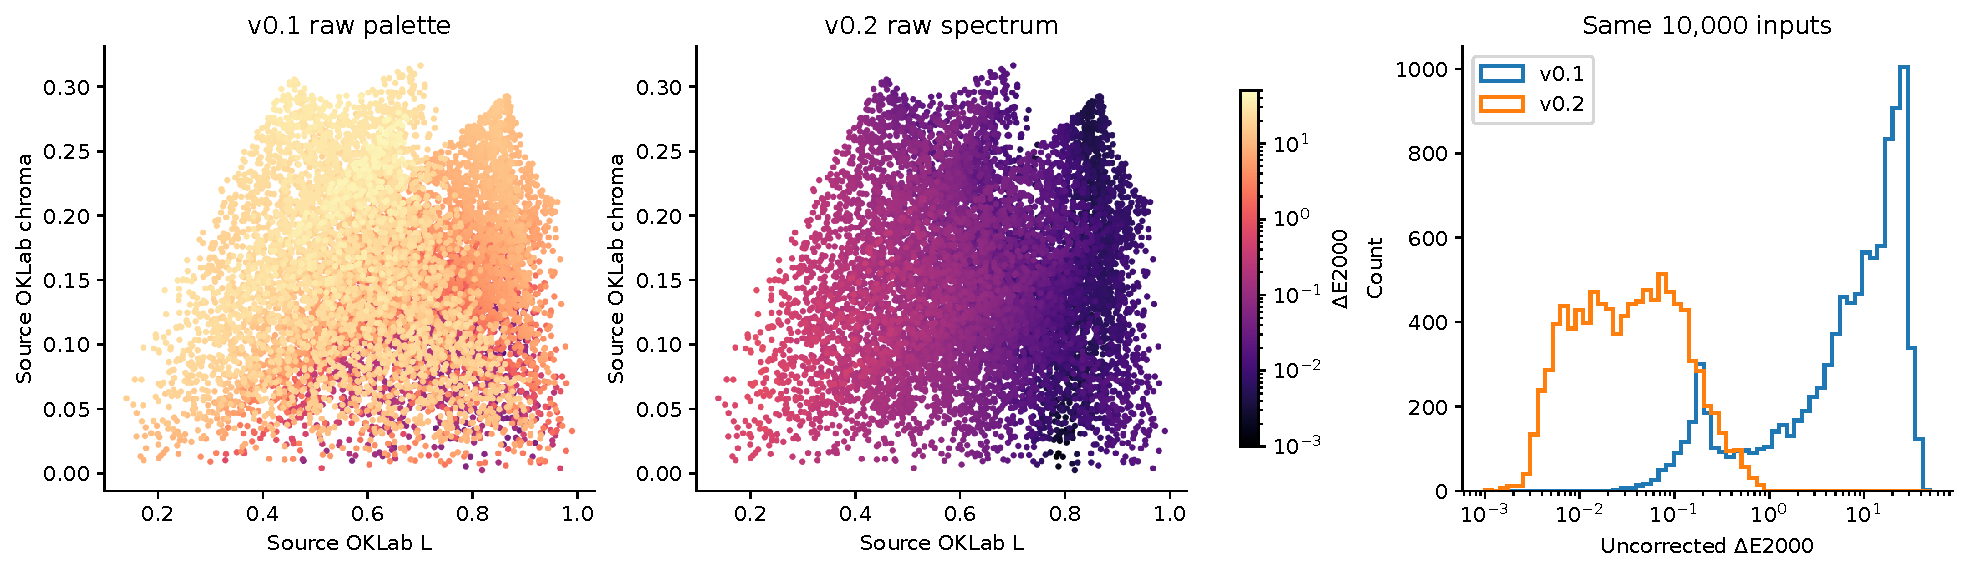
\includegraphics[width=0.94\textwidth,height=0.72\textheight,keepaspectratio]{figures/reconstruction.pdf}
\caption{Uncorrected reconstruction on the same 10,000 colors. The
shared color scale exposes both the earlier palette's large errors and
the new spectrum's remaining dark-region errors.}
\end{figure*}

The new fast/reference mixture error has mean 0.00352, P95 0.013 and
maximum 0.0999 CIEDE2000. The 10 nm choice substantially reduces the 20
nm and 40 nm outliers. A 1 nm evaluation of the interpolated fitted
spectra differs from the 5 nm reference by mean 0.026 and maximum 0.268.
This control prevents treating the chosen reference grid as an exact
continuum solution.

\begin{table*}[t]
\caption{Sampling discrepancy from the 5 nm computational reference.}
\centering\small
\begin{tabular}{@{}llll@{}}
\toprule\noalign{}
Spacing (nm) & Mean & P95 & Max \\
\midrule\noalign{}

\bottomrule\noalign{}

1 & 0.026 & 0.0861 & 0.268 \\
5 & 0 & 0 & 0 \\
10 & 0.00352 & 0.013 & 0.0999 \\
20 & 0.087 & 0.341 & 2.35 \\
40 & 0.849 & 2.84 & 10.5 \\
\end{tabular}
\end{table*}

Only 0.46\% of the new random mixtures require gamut compression. Their
unmapped channel range is {[}-0.01698, 1.00485{]}. This fraction
measures an implementation intervention, not whether an in-gamut result
is physically correct.

\hypertarget{mixing-and-tint-behavior}{%
\subsection{7.2 Mixing and tint
behavior}\label{mixing-and-tint-behavior}}

The dark blue/yellow failure is resolved under the green-dominant
diagnostic; cyan/magenta becomes distinctly blue-violet and red/white
becomes pinker. The full canonical gradients are shown without omitting
unsuccessful or less favorable cases. New red/blue is less saturated
than the older dark purple, and the pure-yellow/pure-blue midpoint is
darker. These are tradeoffs rather than unqualified improvements.

\begin{table*}[t]
\caption{Canonical half-mixture colors.}
\centering\small
\begin{tabular}{@{}lll@{}}
\toprule\noalign{}
Pair & v0.1 sRGB8 & v0.2 sRGB8 \\
\midrule\noalign{}

\bottomrule\noalign{}

yellow + blue & (49, 144, 112) & (101, 152, 94) \\
red + blue & (88, 0, 71) & (106, 57, 98) \\
red + yellow & (242, 118, 14) & (244, 106, 37) \\
cyan + magenta & (148, 101, 130) & (109, 93, 186) \\
magenta + yellow & (237, 120, 116) & (236, 105, 83) \\
black + white & (141, 141, 141) & (166, 166, 166) \\
red + green & (137, 100, 39) & (116, 93, 53) \\
blue + orange & (103, 87, 91) & (108, 114, 83) \\
yellow + purple & (162, 130, 134) & (187, 126, 84) \\
blue + white & (107, 188, 255) & (135, 169, 255) \\
red + white & (255, 166, 124) & (250, 131, 139) \\
extreme + yellow + blue & (60, 174, 124) & (86, 138, 100) \\
official + default & (73, 97, 107) & (99, 138, 68) \\
\end{tabular}
\end{table*}

\begin{figure*}[t]
\centering
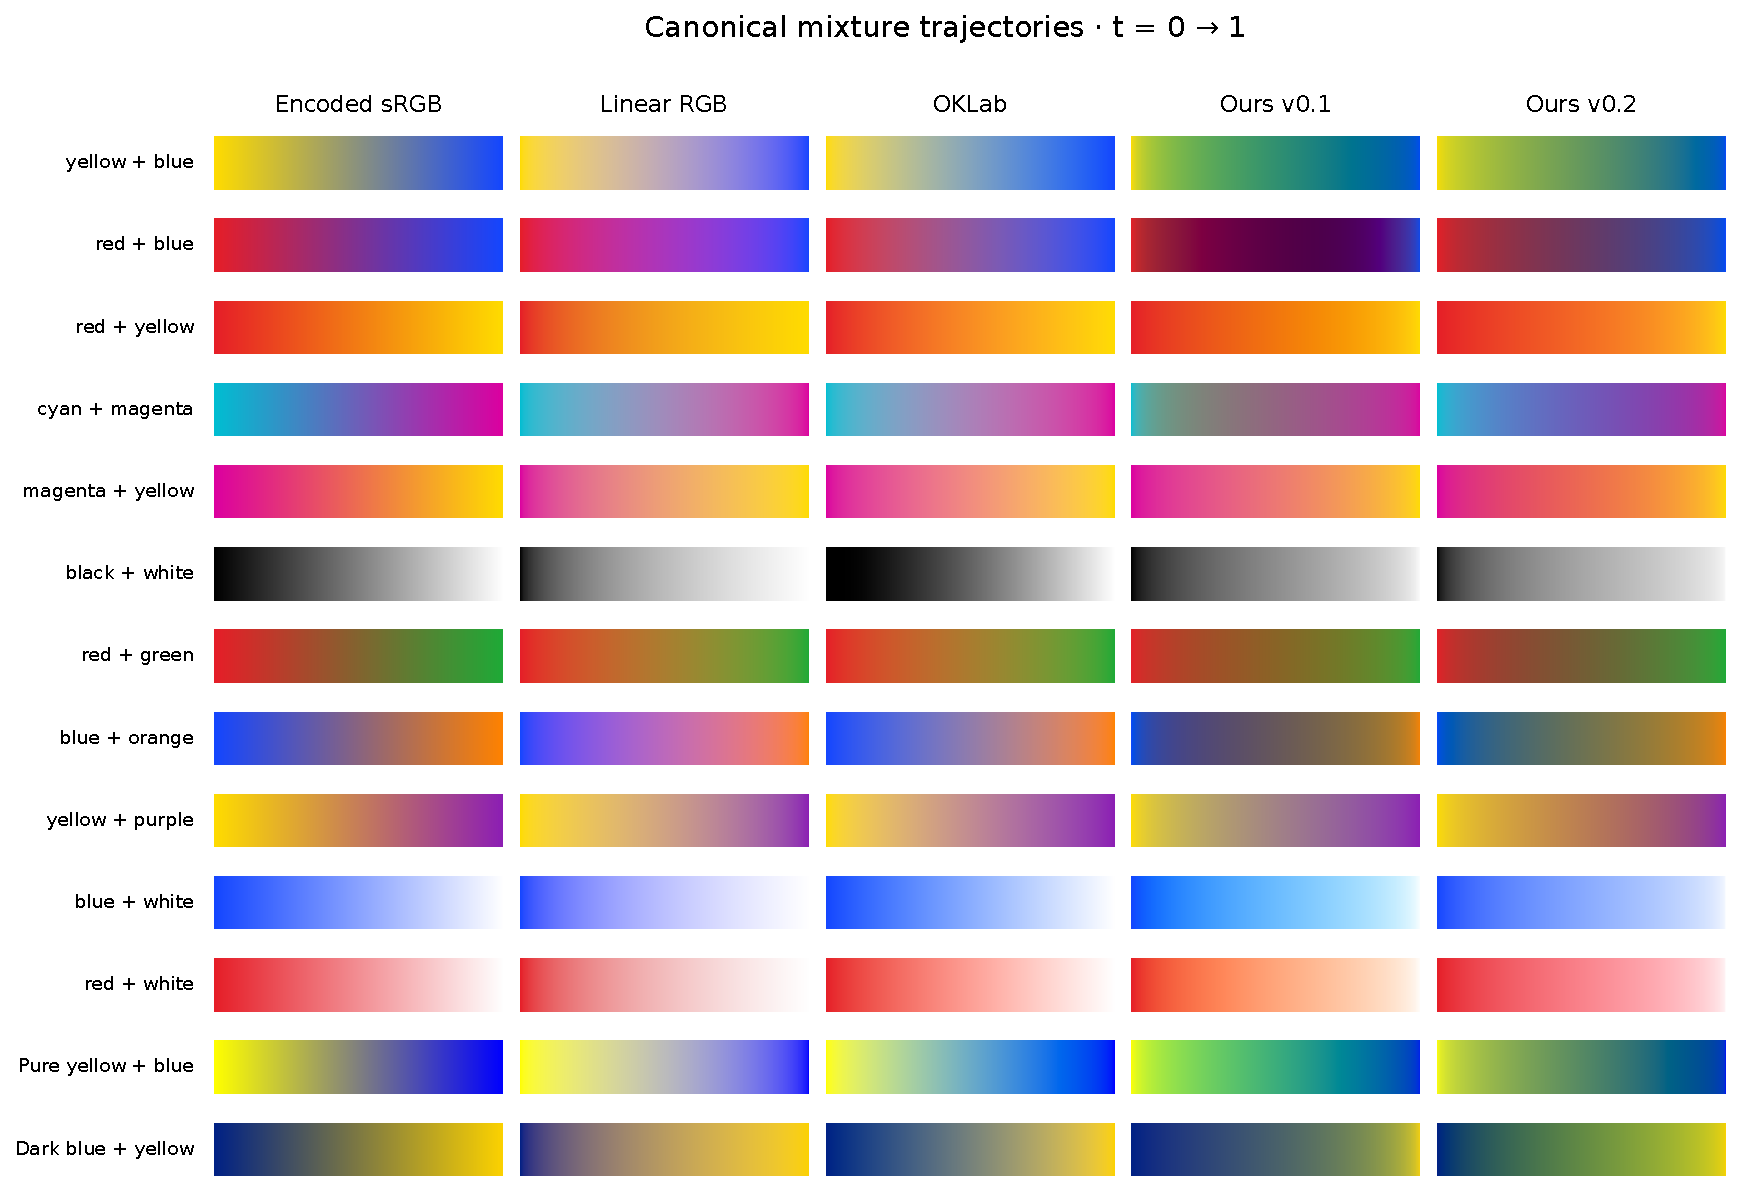
\includegraphics[width=0.94\textwidth,height=0.72\textheight,keepaspectratio]{figures/comparisons.pdf}
\caption{All canonical gradients, with encoded-sRGB, linear-light,
perceptual and both pigment models. No panel represents measured paint.}
\end{figure*}

The held-out green-dominant frequency rises from 38.4\% to 80.8\%. The
remaining non-green outcomes show that the rule is not guaranteed for
arbitrary blue/yellow inputs. In the common eligible white-tint set,
median hue shift decreases from 4.21 to 2.34 degrees, and P95 decreases
from 35.6 to 10.4 degrees. Both models show monotone sampled luminance
for the tested tints. This supports improved hue retention in the
declared diagnostic, not a claim about any named white pigment.

\begin{figure*}[t]
\centering
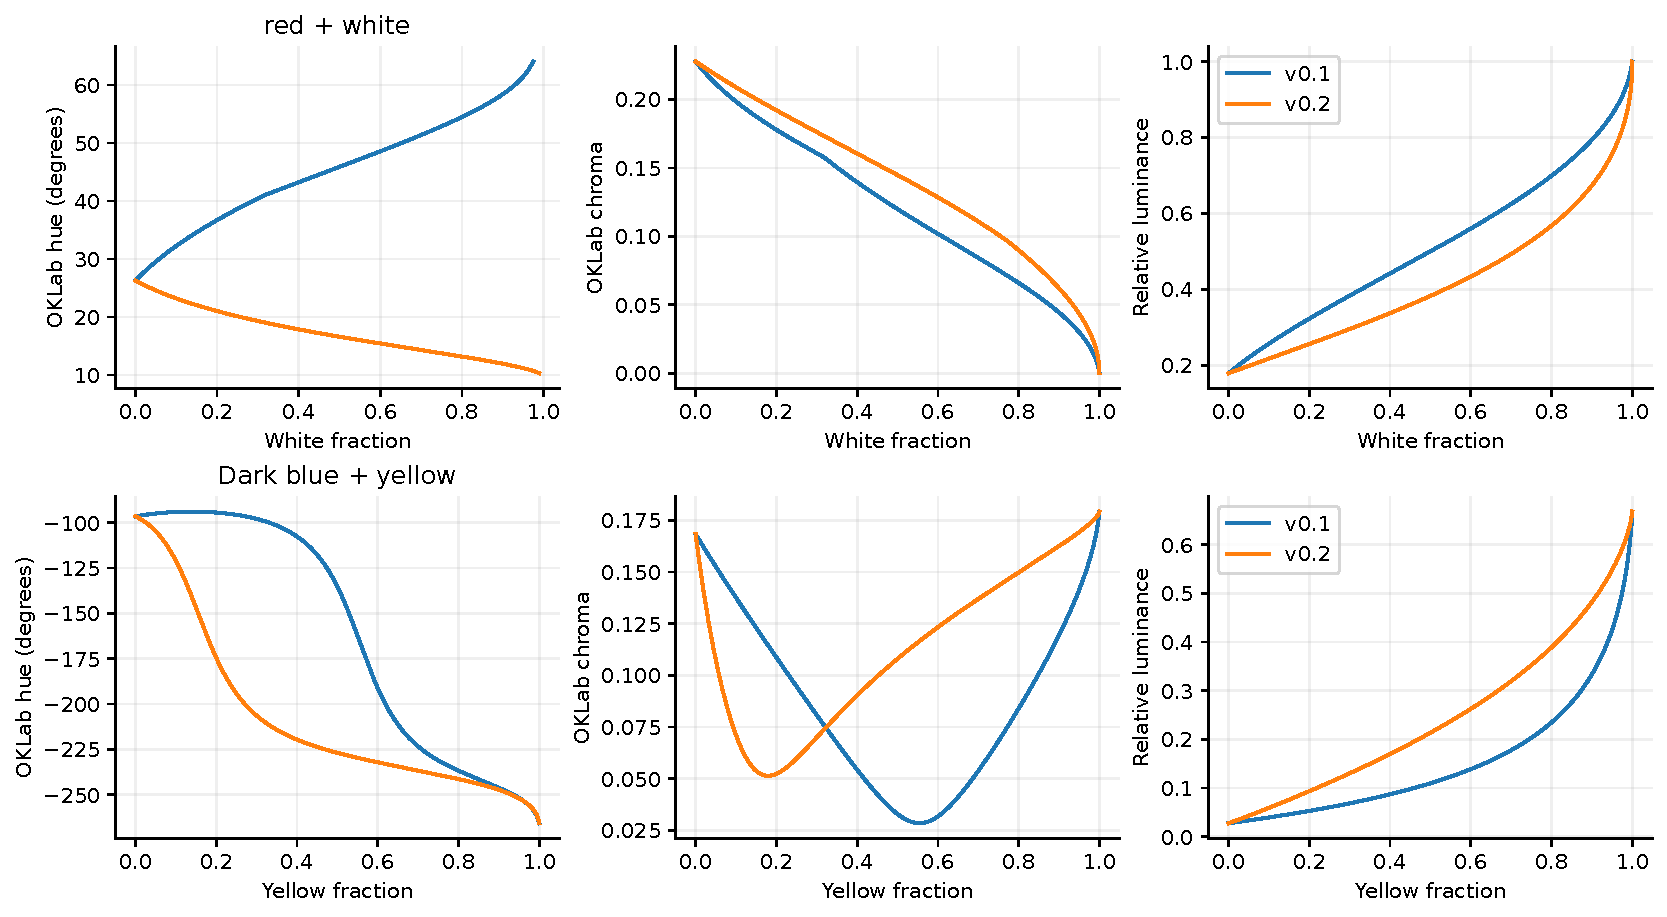
\includegraphics[width=0.94\textwidth,height=0.72\textheight,keepaspectratio]{figures/trajectories.pdf}
\caption{Hue, chroma and luminance for red/white and the
dark-blue/yellow failure case. Hue is omitted near neutral colors, where
it is unstable.}
\end{figure*}

\hypertarget{smoothness-and-sensitivity}{%
\subsection{7.3 Smoothness and
sensitivity}\label{smoothness-and-sensitivity}}

The maximum adjacent random-trajectory step decreases from 1.59 to 1.17
\ensuremath{\Delta}EOK100 at \(\Delta t=0.001\). The new P99 of per-trajectory maxima is
0.929 versus 0.815 previously, so the tail does not improve uniformly.
The largest midpoint response to an encoded-channel perturbation falls
from 0.0132 to 0.00169 \ensuremath{\Delta}EOK100. This is consistent with removing
ambiguous inverse recipes, but finite sampling cannot certify a global
Lipschitz bound.

Pure black remains a special case. Its first black/white step has 10
\ensuremath{\Delta}EOK100; linear RGB interpolation gives 10 under the same sampling. The
new trajectory converges toward black as t decreases, and sampled linear
luminance increases monotonically. An initial test imposing an arbitrary
universal bound of 2 \ensuremath{\Delta}EOK100 per step failed here. We retain that
negative finding and separate continuity from perceptual speed. No
discontinuity or nonfinite value was observed in the evaluated
trajectories.

\hypertarget{runtime-and-state-cost}{%
\subsection{7.4 Runtime and state cost}\label{runtime-and-state-cost}}

\begin{table*}[t]
\caption{Single-thread runtime; cached states omit input encoding.}
\centering\small
\begin{tabular}{@{}lll@{}}
\toprule\noalign{}
Operation & Median ns & Million/s \\
\midrule\noalign{}

\bottomrule\noalign{}

sRGB & 15.6 & 64 \\
linear RGB & 148 & 6.75 \\
OKLab & 272 & 3.67 \\
v0.1 RGB & 572 & 1.75 \\
v0.2 RGB & 719 & 1.39 \\
v0.2 cached & 229 & 4.37 \\
v0.2 reference & 1.87e+03 & 0.534 \\
v0.1 cached & 182 & 5.5 \\
\end{tabular}
\end{table*}

The revised fast path processes 1.39 million complete RGB mixtures per
second and 4.37 million cached mixtures per second on this host. It is
slower than the old default in both modes. Its reference is much cheaper
than the preceding optimizer-based reference because reconstruction is
explicit; this is an architectural change, not merely a compiler
optimization. The larger state is an important integration cost. The
measurements support interactive use for many workloads, but not a
blanket claim that per-pixel spectral storage or every application is
practical.

\begin{figure*}[t]
\centering
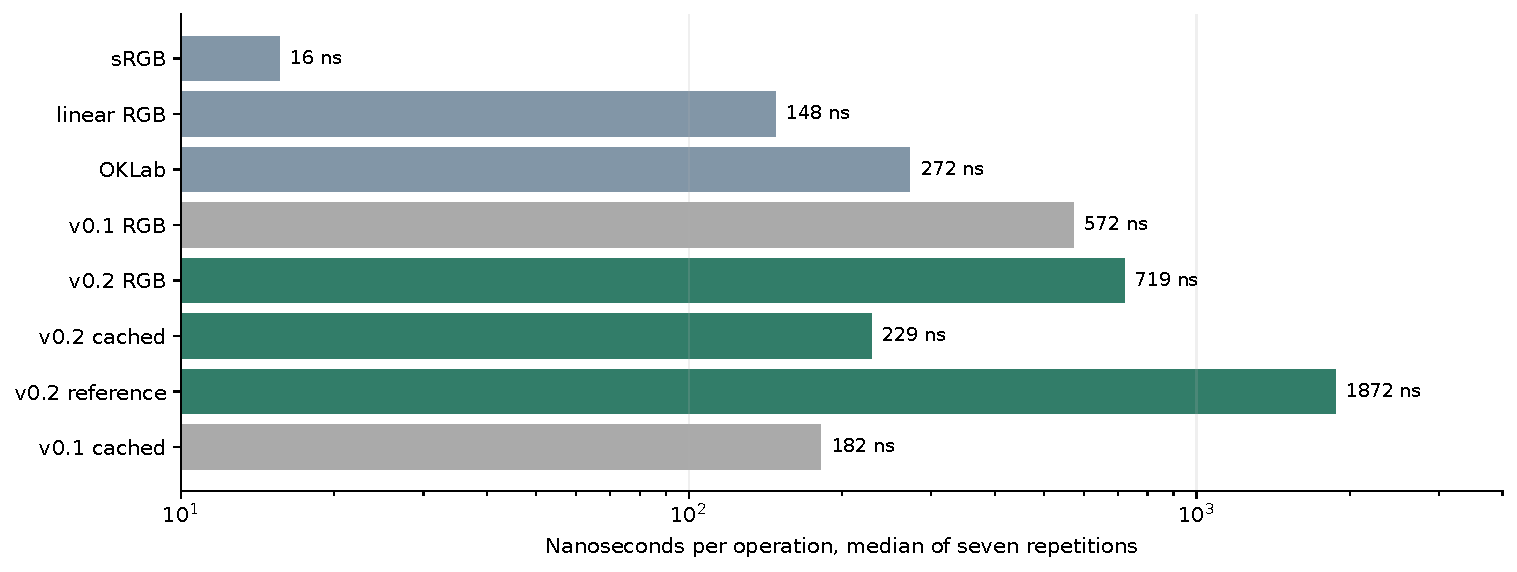
\includegraphics[width=0.94\textwidth,height=0.72\textheight,keepaspectratio]{figures/performance.pdf}
\caption{Measured median operation costs. Cached rows omit input
encoding; all mixing rows include final display conversion.}
\end{figure*}

\hypertarget{ablation-studies-and-negative-findings}{%
\section{8. Ablation studies and negative
findings}\label{ablation-studies-and-negative-findings}}

Refitting the original eight-pigment palette with the new reflectances,
while retaining finite-palette K/S mixing and nonlinear inversion, did
not solve the diagnostic failures. Its half black/white result was
{[}35,35,35{]}, and the dark-blue/yellow midpoint remained teal. This
does not prove that no finite palette could work; it shows that improved
isolated-color coverage alone was insufficient for the tested
construction.

Constant scattering combined with near-black spectra produced excessive
absorption in black/white mixing. Conversely, pure per-band
normalization (\(\beta=1\)) improved some violet mixtures but reduced
the frequency of convincing green blue/yellow results. The selection
sweep shows the conflict between green-family coverage and tint hue
retention. The chosen \(\beta=0.5\) is a compromise; \(\beta=0.25\)
retains more green-family results but shifts tint hues more. White
strengths 1, 2 and 4 all preserve isolated reflectance, yet produce
different tint trajectories. This is a direct demonstration of the
optical-strength ambiguity.

\begin{figure*}[t]
\centering
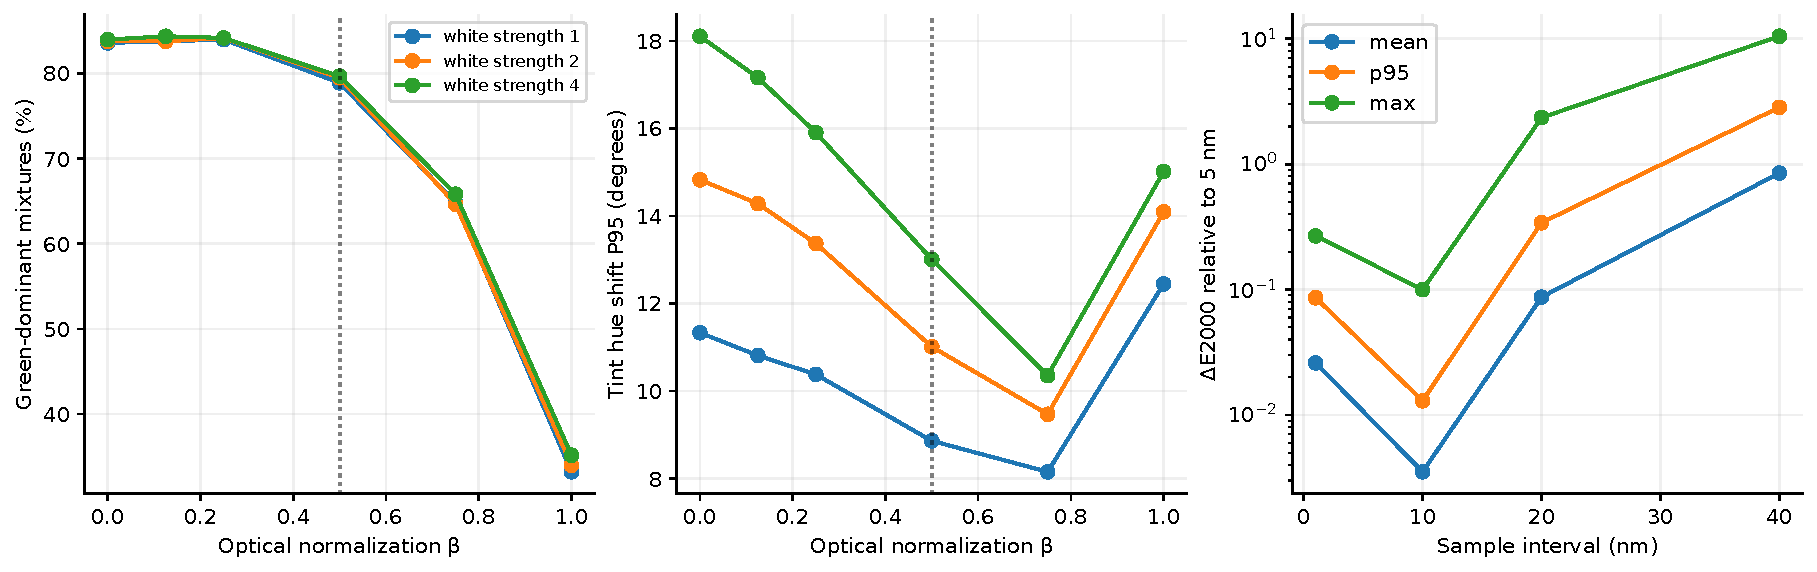
\includegraphics[width=0.94\textwidth,height=0.72\textheight,keepaspectratio]{figures/ablations.pdf}
\caption{Selection-set normalization and white-strength ablations, plus
held-fixed-spectrum sampling error. The dotted line marks the chosen \ensuremath{\beta};
these curves are design diagnostics, not paint-fit errors.}
\end{figure*}

Logit smoothness values 0.0001, 0.001, 0.01 and 0.03 were recorded.
Larger values improved spectral smoothness at the expense of
saturated-anchor fidelity. The selected value was not fit to a target
set of real mixtures. Residual removal has a much smaller effect on
source accuracy after the revision, but the residual remains useful for
bounded black/white and sampling error. Eliminating it entirely would
break exact RGB compatibility without establishing physical correctness.

The 20 nm approximation offers fewer samples but larger outliers; 40 nm
is substantially worse. The 10 nm choice favors accuracy while retaining
measured interactive throughput. We did not add a second LUT, neural
approximation or explicit SIMD layer because the continuous encoder
already met the selected runtime target and avoided an additional
approximation to validate.

\hypertarget{comparison-with-other-engines}{%
\section{9. Comparison with other
engines}\label{comparison-with-other-engines}}

On the 39 frozen Mixbox observations, our mean difference decreases from
13.5 to 6.92 CIEDE2000; the new maximum remains 23.2. Spectral.js
differs from those same observations by mean 7.86. Across all 5,213
Spectral.js samples, the old/new differences are 13.1 and 6.49
respectively. These reductions are descriptive and were measured after
selection. They do not demonstrate equivalence, establish a ranking
against real paint, or justify adapting our coefficients to proprietary
outputs.

Mixbox captures have JPEG uncertainty and a small selected sample count.
Spectral.js produces quantized 8-bit API outputs under specified
settings. The paired endpoints and t values make the experiment useful
for visual comparison, while the different acquisition methods limit
numerical interpretation. The supplement shows the complete external
comparison and all retained metadata. A proper physical validation would
instead specify paints, amounts, preparation, thickness, substrate and
illumination, then compare held-out measured mixtures.

\hypertarget{discussion-and-limitations}{%
\section{10. Discussion and
limitations}\label{discussion-and-limitations}}

The revision demonstrates that mathematical work can remove large
artificial reconstruction errors and improve declared visual diagnostics
without new experimental paint data. It cannot determine the correct
metamer or strength for an unknown RGB source. Good endpoint
colorimetry, green midpoints, hue retention and similarity to other
software are different criteria; none substitutes for physical
validation.

The new reconstruction basis spans display colors more effectively
because it is designed for that purpose. Its spectra and strengths are
synthetic and may not correspond to manufacturable pigments. The optical
prior favors bounded, tractable behavior and was selected on a limited
diagnostic family. Results remain dependent on the observer, illuminant,
wavelength interval, reflectance bounds, smoothing and gamut policy. The
method does not model real metameric changes under different lights.

Infinite-thickness diffuse optics omit film thickness, translucent
glazing, gloss, fluorescence, metallic and interference pigments,
granulation, binder-dependent behavior, particle-size effects and
spatial transport. These limitations are relevant to the implemented
equations, rather than a claim that a different K--M formulation could
never address some of them. The positive spectral floor and numerical
white normalization are additional modeling approximations.

The reference is a high-precision evaluation of our model, not
experimental ground truth. Tests establish finite-sample properties and
selected algebraic invariants. There was no human preference study.
Reduced tint hue shift is an explicit design preference; real paint can
shift hue during tinting. Random encoded-RGB tests overrepresent some
color regions and underrepresent actual painting workflows. The state
size and slower full-RGB path may matter more than the improved
diagnostics in a memory-limited application.

\hypertarget{reproducibility-and-future-work}{%
\section{11. Reproducibility and future
work}\label{reproducibility-and-future-work}}

\texttt{python3\ tools/reproduce.py} reads the root TOML, fits the
anchors, builds and tests Rust, reruns the experiments, regenerates
figures and tables, and renders the manuscript when Pandoc/TeX are
available. The package pins Python dependencies, records compiler/CPU
configuration and seeds, and stores raw samples and optimizer results.
The legacy implementation, paper and reproduction workflow are
preserved. External comparisons use frozen observations by default; they
do not silently query a changing live service.

Original code is MIT OR Apache-2.0. Attributed CIE-derived data and
derived numerical assets carry CC BY-SA 4.0 notices, so the complete
distribution is not exclusively MIT-licensed. The generated basis is
inspectable CSV and Rust arrays, not unexplained binary data. No
proprietary Mixbox artifact is required to build, fit or execute the
engine.

Useful next work includes state compression validated against the
current optical state, explicit SIMD/GPU kernels, WASM execution
measurements, artist evaluation and workload-specific caching. Measured
paint data, if later available, could define a separate calibrated
material mode rather than retroactively making arbitrary RGB inversion
unique. Finite-layer optics and substrate effects should be introduced
with their own validation instead of adjusting opaque mixing heuristics
to mimic glazing.

\hypertarget{conclusion}{%
\section{12. Conclusion}\label{conclusion}}

Replacing a constrained finite-palette inverse with continuous spectral
reconstruction substantially reduces raw color mismatch and improves the
selected blue/yellow and tint diagnostics. The chosen optical-strength
normalization is essential: better reflectance reconstruction alone did
not provide suitable mixture behavior. The fast implementation retains
low error against its own reference and measured interactive throughput,
with larger cached state and slower mixing than the previous LUT model.
Residual correction ensures RGB compatibility, while the improved
uncorrected results reduce reliance on that correction. The result is a
reproducible, physically motivated painting surrogate whose assumptions
and remaining failures are explicit; it is not a calibrated predictor of
unspecified real paints.

\hypertarget{references}{%
\section*{References}\label{references}}
\addcontentsline{toc}{section}{References}

\hypertarget{refs}{}
\begin{CSLReferences}{1}{0}
\leavevmode\vadjust pre{\hypertarget{ref-burns2020}{}}%
Burns, Scott Allen. 2020. {``Numerical Methods for Smoothest Reflectance
Reconstruction.''} \emph{Color Research and Application} 45: 8--21.
\url{https://doi.org/10.1002/col.22437}.

\leavevmode\vadjust pre{\hypertarget{ref-colour}{}}%
Colour Developers. n.d. {``Colour: Colour Science for Python, Version
0.4.6.''} \url{https://github.com/colour-science/colour}.

\leavevmode\vadjust pre{\hypertarget{ref-curtis1997}{}}%
Curtis, Cassidy J., Sean E. Anderson, Joshua E. Seims, Kurt W.
Fleischer, and David H. Salesin. 1997. {``Computer-Generated
Watercolor.''} In \emph{Proceedings of SIGGRAPH}, 421--30.
\url{https://grail.cs.washington.edu/projects/watercolor/}.

\leavevmode\vadjust pre{\hypertarget{ref-gossett2004}{}}%
Gossett, Nathan, and Baoquan Chen. 2004. {``Paint Inspired Color Mixing
and Compositing for Visualization.''} In \emph{IEEE Symposium on
Information Visualization}, 113--18.
\url{https://doi.org/10.1109/INFOVIS.2004.52}.

\leavevmode\vadjust pre{\hypertarget{ref-haase1992}{}}%
Haase, Chet S., and Gary W. Meyer. 1992. {``Modeling Pigmented Materials
for Realistic Image Synthesis.''} \emph{ACM Transactions on Graphics} 11
(4): 305--35. \url{https://doi.org/10.1145/146443.146452}.

\leavevmode\vadjust pre{\hypertarget{ref-hebert2015}{}}%
Hébert, Mathieu, and Roger D. Hersch. 2015. {``Review of Spectral
Reflectance Models for Halftone Prints: Principles, Calibration, and
Prediction Accuracy.''} \emph{Color Research and Application}.
\url{https://doi.org/10.1002/col.21907}.

\leavevmode\vadjust pre{\hypertarget{ref-cied65}{}}%
International Commission on Illumination. 2019a. {``{CIE} Standard
Illuminant {D65}.''} \url{https://doi.org/10.25039/CIE.DS.hjfjmt59}.

\leavevmode\vadjust pre{\hypertarget{ref-cieobserver}{}}%
---------. 2019b. {``Colour-Matching Functions of {CIE} 1931 Standard
Colorimetric Observer.''}
\url{https://doi.org/10.25039/CIE.DS.xvudnb9b}.

\leavevmode\vadjust pre{\hypertarget{ref-jakob2019}{}}%
Jakob, Wenzel, and Johannes Hanika. 2019. {``A Low-Dimensional Function
Space for Efficient Spectral Upsampling.''} \emph{Computer Graphics
Forum} 38 (2). \url{https://doi.org/10.1111/cgf.13626}.

\leavevmode\vadjust pre{\hypertarget{ref-kubelka1948}{}}%
Kubelka, Paul. 1948. {``New Contributions to the Optics of Intensely
Light-Scattering Materials. Part i.''} \emph{Journal of the Optical
Society of America} 38 (5): 448--57.
\url{https://doi.org/10.1364/JOSA.38.000448}.

\leavevmode\vadjust pre{\hypertarget{ref-kubelka1931}{}}%
Kubelka, Paul, and Franz Munk. 1931. {``Ein Beitrag Zur Optik Der
Farbanstriche.''} \emph{Zeitschrift f{ü}r Technische Physik} 12:
593--601.

\leavevmode\vadjust pre{\hypertarget{ref-ottosson2020}{}}%
Ottosson, Björn. 2020. {``A Perceptual Color Space for Image
Processing.''} \url{https://bottosson.github.io/posts/oklab/}.

\leavevmode\vadjust pre{\hypertarget{ref-sharma2005}{}}%
Sharma, Gaurav, Wencheng Wu, and Edul N. Dalal. 2005. {``The {CIEDE2000}
Color-Difference Formula: Implementation Notes, Supplementary Test Data,
and Mathematical Observations.''} \emph{Color Research and Application}
30 (1): 21--30. \url{https://doi.org/10.1002/col.20070}.

\leavevmode\vadjust pre{\hypertarget{ref-smits1999}{}}%
Smits, Brian. 1999. {``An {RGB}-to-Spectrum Conversion for
Reflectances.''} \emph{Journal of Graphics Tools} 4 (4): 11--22.
\url{https://doi.org/10.1080/10867651.1999.10487511}.

\leavevmode\vadjust pre{\hypertarget{ref-sochorova2021}{}}%
Sochorová, Šárka, and Ondřej Jamriška. 2021. {``Practical Pigment Mixing
for Digital Painting.''} \emph{ACM Transactions on Graphics} 40 (6):
234:1--11. \url{https://doi.org/10.1145/3478513.3480549}.

\leavevmode\vadjust pre{\hypertarget{ref-spectraljs}{}}%
Spectral.js contributors. n.d. {``Spectral.js: Realistic Color Mixing,
Version 3.0.0.''} \url{https://github.com/rvanwijnen/spectral.js}.

\leavevmode\vadjust pre{\hypertarget{ref-tan2017}{}}%
Tan, Jianchao, Stephen DiVerdi, Jingwan Lu, and Yotam Gingold. 2017.
{``Pigmento: Pigment-Based Image Analysis and Editing.''}
\url{https://arxiv.org/abs/1707.08323}.

\leavevmode\vadjust pre{\hypertarget{ref-csscolor}{}}%
World Wide Web Consortium. n.d. {``{CSS} Color Module Level 4.''}
\url{https://www.w3.org/TR/css-color-4/}.

\end{CSLReferences}

\end{document}
